\documentclass[12pt]{article}

\usepackage{sbc-template}
\usepackage[normal]{subfigure}  % permite utilizar subfiguras
\usepackage{graphicx,url}
\usepackage{amssymb}
\usepackage{rotating}
%\usepackage[brazil]{babel}   
\usepackage[latin1]{inputenc}  
\usepackage{booktabs}
\usepackage{multirow}
\usepackage{color}




\newcommand{\e}{\emph}
\renewcommand{\b}{\textbf}
\renewcommand{\t}{\textsc}
%\newcommand{\t{Logicamente}}{\textsc{Logicamente}~}
\newcommand{\noi}{\noindent}
\newtheorem{mydef}{Defini��o}


\sloppy

%\b{\scriptsize{\color{red}{Patrick says:THERE IS MANY ERRORS TO CORRECT IN THE PAPER}\color{black}}}

\title{ The \t{Logicamente}: collaborative challenges and benefits of a tool for teaching and learning Logic \footnote{The authors acknowledge financial support from CNPq/CAPES. Thanks to all students of Computer Science and Computer Engineering who contributed to the project \t{Logicamente} for a few semesters in the discipline of Logic Applied to Computer on Federal University of Rio Grande do Norte. Indeed, thanks to Prof. Jo�o Marcos, for all his attention to making it possible, to create and advise this project.}}

%\footnote{Agradecimentos ao CNPq, pela bolsa de financiamento de mestrado para X, ao Prof. Y, por toda sua aten��o ao criar e orientar este projeto, ao CNPq/UFRN, pela bolsa de inicia��o cient�fica para Z, que tamb�m merece nossa gratid�o pela sua dedica��o e pelo �timo trabalho de implementa��o.}
\author{ Patrick Terrematte\inst{1}, Fabr�cio Costa\inst{1} }


\address{ Federal University of Rio Grande do Norte (UFRN)\\  Department of Informatics and Applied Mathematics (DIMAp)\\
Group of Logic, Language, Information, Theory and Applications (LoLITA) \\  59078-970 -- Natal -- RN -- Brasil \\ \url{terrematte@ppgsc.ufrn.br}, \url{fabriciocscte@ppgsc.ufrn.br}}
%\address{ Departamento [Omitido para revis�o] -- Universidade -- \\  Brasil }

\begin{document} 

\maketitle


\begin{abstract}
Logic is a subject offered to many undergraduate courses with different focal points.  For most of those courses, it is remarkable how Logic represents a pedagogic challenge for both teachers and students, and the recorded number of cases of failures and of discontinuity is often high.  Given the need to provide a solid basis in the subject, we propose a set of Learning Object (LO) for teaching Logic Applied to Computer Science: the \t{Logicamente}\footnote{Is partiality avaliable from \url{http://www.lolita.dimap.ufrn.br/Logicamente}.}.  The tools that integrate the system aim to illustrate fundamental concepts and algorithms from Logic, as well as to allow students to conduct interactive practical experiments involving the understanding of those concepts.\\
\b{Key-words:} Learning Objects. Teaching Logic. Logic.
\end{abstract}
     
\begin{resumo} 
A disciplina de L�gica � oferecida por diversos cursos de gradua��o com diferentes focos de aplica��o.  Para a maioria desses cursos, � not�vel como a disciplina representa um desafio pedag�gico para os professores e os alunos de gradua��o, assim como � frequentemente alto o n�mero de trancamentos e reprova��es registrados.  Diante da necessidade de uma forma��o s�lida dos alunos na disciplina, propomos um conjunto de Objetos de Aprendizagem (OA) para o ensino de L�gica Aplicada � Computa��o: o \t{Logicamente}. As ferramentas que integram o sistema visam a ilustrar conceitos e algoritmos fundamentais da L�gica e a permitir que os estudantes fa�am experimentos pr�ticos envolvendo a compreens�o desses conceitos de forma interativa.\\
\b{Palavras-chave:} Objetos de Aprendizagem. Ensino de L�gica. L�gica.
\end{resumo}

\section{Introduction: Main aspects of teaching and learning Logic}

\begin{flushright}
\scriptsize
``\e{Logic: The art of thinking and reasoning in strict accordance \\
with the limitations and incapacities of the human misunderstanding.}'' \\
\t{--- Ambrose Bierce} \\
\e{The Collected Works of Ambrose Bierce (1911), Vol. 7, The Devil's Dictionary,  196. }
\end{flushright}



\noi  The logic has not been sufficient emphasis on computer courses. We note that there are some talents working in universities in that area. But why is it important to study logic and why it has not had their due importance? In \cite{Barland2000} are mentioned two points that is happening in computer courses. The first is the myth that comes from students, which argue that knowledge of logic will not be useful in their professional careers. The second point is the part of teachers and educational institutions. Often they were not prepared, teaching in a superficial way the content of logic and in other cases the actual course curriculum has trouble putting the logic with a secondary issue within a matter of discrete mathematics, spending a few weeks to teach all content on logic. 


Beyond thoses reasons, the logical concepts are not trivial to understand, then generating a digression on this subject. Aimed to gather some solutions \cite{Barland2000} brings several points illustrating why we must study logic. The main ones are: Software developers must analyze the behavior of their programs; circuit minimization and equivalence checking Rely on the logical equivalence of designs; Establishing protocol correctness Requires a specification language and verification Corresponding framework. These are some of the many uses of logic.

Seen it, we have pointed out problems in the teaching logic, both attributed to disinterest and lack of proper training of educators.The project \t{Logicamente} has as main goal treat logic as a friendly discipline, bringing an interactive way to teach with content adaptation making it easier to learn logic. In this sense we see the power of the Semantic Web and ontologies with regard to learning objects.

We may have learning material tailored to the needs of each student through an ontology that establishes the connection between these needs and the learning materials. Among many challenges, we focus now on study materials for learning objects, seeking efficiency in search, recovery and adaptation of teaching materials. We aim to further that learning objects are based on ontologies. We believe that virtual environments can benefit from the use of semantic web based in ontologies.


	\subsection{Learning Logics Tools: Challenge, Benefits and Oportunities}

\noi The project \t{Logicamente} is developed aiming to explore the advantages of web applications on teaching of logic, implementing some LOs  to perform tasks such as: the automatic generation of formulas with the desired complexity, the configuration of a language and to develop new connectives, the translation between different syntaxes, the construction of truth tables and tableaux of formulas, the interactive presentation of formulas in the form of trees, the implementation of the method of resolution for classical logic, the search for models or counter-models and moreover, the use of an assistant for the demonstration of theorems. \footnote{For a better understanding of the concepts of logic implemented in Logic, cf. \cite{Barwise2002,Dalen2004}.}

Thus, we expose a set of interactive LOs gathering tools to support teaching of Logic Applied to Computation. Our goal is to produce integrated instruments that illustrate fundamental concepts and algorithms of logic, allowing students to make practical and pedagogical experiments. Finally, we point out some methodological expectations and what we intend to perform further work to make the \t{Logicamente} a Virtual Learning Environment of Logic.


Currently, the conventional curricula in our universities prefer students with an intuitive learning style, verbal, deductive, reflective and sequential, as opposed to those students that learn by other ways \cite{Barland2000,Felder1988}. Adding this to the lack of solid basic knowledge of the begginer undergraduate students and the precarious learning resources available,  is not surprising that there is a high failure rate and locking of the discipline of Logic Applied Computer in several universities and technology centers.

To solve thoses problems in the teaching of logic, we invested in a more sensory learning style, visual, inductive, active and comprehensive, aimed  professional training able to meet more effectively the needs of the industrial sector and academic community.


%ADD outros sistemas: ORGANON... 

\begin{table}[ht]
\scriptsize
  \centering
  \caption{List of learning tools Logic}
    \begin{tabular}{|r|c|c|r|c|}
    \addlinespace
    \toprule
    \# & NAME & CONTENT  & IMPLEMENTION & WEB\\
	\midrule 
   1 & \e{Akka}  & Prop. and $1^{st}$ Order; Kripke Models & Java Applets & *  \\ \hline
   2 & \e{Apros} & Prop. and $1^{st}$ Order; Natural Deduction   & Java Web Start & *  \\ \hline
   3 & \e{ASA-CalcPro} & Prop; Tableaux; Truth Table    & Java  & -  \\  \hline   
   4 & \e{Comp. Aristotelian Logic} & Aristotelian Logic    & PHP   & $\checkmark$  \\  \hline
   5 & \e{Expression Evaluator} & Prop. and $1^{st}$ Order; Expression Evaluator & Perl/cgi & $\checkmark$  \\ \hline
   6 & \e{JAPE}  & Prop. and $1^{st}$ Order; Natural Deduction   & Java  &  - \\ \hline
   7 & \e{LoTREC} &  Prop. and $1^{st}$ Order; Modal &  Java Applets  & * \\ \hline
   8 & \e{Pandora} & Prop. and $1^{st}$ Order; Natural Deduction    & Java Applets &* \\ \hline
   9 & \e{Possible World Creation} & Prop.; Modal & Flash & $\checkmark$ \\ \hline
   10 & \e{ProofWeb} & Web Assistent-Proof; Natural Deduction & Ocaml & $\checkmark$  \\ \hline
   11 & \e{ORGANON} &   Prop. and $1^{st}$ Order; Semantic; Tableaux and Truth Table & Servlets &  $\checkmark$ \\ \hline 
   12 & \e{Tarski's World} &  Prop. and $1^{st}$ Order; Semantic and Tableaux   & Java  & * \\\hline
   13 & \e{Fitch} &  Prop. and $1^{st}$ Order; Natural Deduction  & Java  & * \\\hline
   14 & \e{Boole} & Prop. ; Truth Table  & Java  & * \\\hline
   15 & \e{The Daemon Proof Checker} & Prop. and $1^{st}$ Order; Model Checking; Natural Deduction   & C\#   & -\\ \hline
   16 & \e{Theorem Proving System} & Prop. and $1^{st}$ Order; Natural Deduction  & Lisp     & $\checkmark$ \\ \hline
   17 & \e{Tree Proof Generator}  & Prop. and $1^{st}$ Order e Tableaux  & JavaScript  & $\checkmark$ \\ \hline
   18 & \e{Truth Table Constructor} & Prop.; Truth Table     & Java Applets    & *\\ \hline
   19 & \e{Tableau3} & Prop. and Tableaux   & Java Applets  & * \\ \hline
   20 & \e{DiagVenn1.0} & Prop. and $1^{st}$ Order; Venn Diagrams  & Java Applets & *  \\ \hline
   21 & \e{MAFIA} & Prop. and $1^{st}$ Order; Kripke Models & Java Applets & *\\ \hline\hline
   22 & \t{Logicamente} & Prop. and $1^{st}$ Order; et al. & PHP  & $\checkmark$ \\ \hline\hline
    \bottomrule
    \end{tabular}
\begin{flushleft}
$^{*}$  Parcially avaliable on the Web.  \\
\end{flushleft}
  \label{tab:logictools}
%\end{sidewaystable}
\end{table}

Many support systems to the teaching of logic are avaliable currently, such as those showed in the Table \ref{tab:logictools}. However, most of them are desktop systems, not avaliable on different operating systems, or they are Web applications based on \emph{Java Applets} without store information about the user's session. These systems are restrictive because they need a Java Virtual Machine (JVM) and usually have a low performance execution. Another problem is that these systems are monothematics and cover a very restricted area of the content of Logic (only one or two contents are implemented by each system) and moreover have no challenging activities and does not stimulate the user.



\section{The Virtual Learning Environement: \t{Logicamente}}




\begin{flushright}
\scriptsize
``\e{La puissance de vision qui fait le po�te, \\
et la puissance de d�duction qui fait le savant,...}'' \\
\t{--- Honor� de Balzac} \\
\e{La Recherche de l'Absolu (1834).}
\end{flushright}


\noi A Virtual Learning Environment (VLE) is a computer system designed to support teaching and learning in an educational monitoring mechanism. A VLE should provide a set of tools, such as appraisals, interactive communication, transfer of content management, student activities, tools, tracking exercises, collaborative entries, Wikis and learning modules specific to the content.


The prototype of \t{Logicamente} was initially implemented in 2006, under the idealization and guidance of Prof. Jo�o Marcos, as a final project of the discipline of Logic Applied  to Computing. The goal was to implement a methodology of Problem-Based Learning (PBL) for the implementation of some key concepts of logic. In the following semesters, the project continued to be developed from the collaborative work of students and volunteers, with the opportunity to present papers that explored both the computational aspects of algorithms implementations as well aspects of computer technology applied to education \cite{Vilela2008, Barros2008, Terrematte2009}. The prototype of the home screen can be seen in Figure \ref{fig:proto-home}.


\begin{figure}[htbp]
\centering
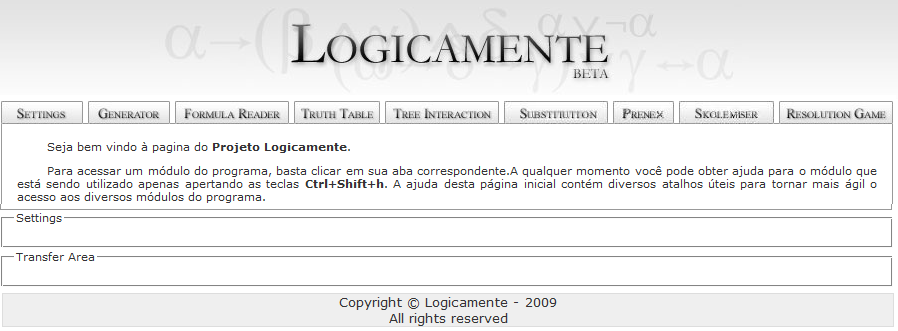
\includegraphics[width=14cm]{f-prototipo-home}
\caption{\t{Logicamente} prototype avaliable currently}
\label{fig:proto-home}
\end{figure}




	\subsection{Some Leaning Objects of \t{Logicamente}}


\noi Currently, we have nine modules, namely: the \e{Settings}, the {Generator}, the \e{Formula Reader}, the \e{Truth-Table Constructor}, the \e{Tree Interaction}, the \e{Substitution Master}, the \e{Prenex Converter}, the \e{Skolemizer} and the \e{Resolution Game}, which will be described below.


\noi $\bullet$	\emph{Settings\/}:  is a module that we can choose which style of notation we want to use. Currently, we can choose the notation style  \e{Infix}, \e{Polish} e \e{Functional}. The notation \e{Infix} is the default -- represented by $\alpha \wedge \beta $ --, while the notation \e{Polish} have conectives preceding the formulas in scope -- $K \alpha \beta$ --  and, the latter case is the notation \e{Function} which represents conectives as functions -- $f(\alpha , \beta)$. Furthermore, its possible to add new connectives by setting his symbol, arity and order of association. The goal is to create new connectives and save them in the database for define new logics. In the picture \ref{fig:settings}, we can find the prototype of this module. 

\noi $\bullet$   \emph{WFF\footnote{ A WFF is a \b{Well Formed Formula}, that mean a sequence of generated according to a formal langage.} Generator\/}: this module is responsible for generate arbitrarily well-formed propositional formulas, according to certain properties entered by the user (number of occurrences of connectives, sentential number of variables and others). With this module, sets of formulas are generate according to the desired complexity and might prepare some exercises automatically with generated formulas. Also the student can generate formulas, put them on the clipboard and analise them in other modules. In the picture \ref{fig:generator}, we observe the generation of three formulas with two connectors and three atoms.

\noi $\bullet$	\e{Formula Reader}: is a module for inserting formulas by the user to the clipboard, to be analised in others modules.

\noi $\bullet$  \e{Truth-Table Constructor}: enables the construction of truth-table and the satisfiability of a collection of formulas, display of all possible states of sentential variables and the complete formula as a whole. Must support, in a second stage, the setting to define new operators for the user, as well for evaluation of formal semantic for certain non-classical logic that can be characterized by interpretations in terms of finite truth tables. In the Figure \ref{fig:truthtable}, we display a truth table for the formula $((p \wedge \neg p) \to q)$.



\begin{figure}[ht]
\center
\subfigure[\e{Settings}]{\label{fig:settings} 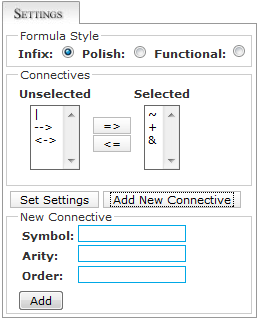
\includegraphics[width=0.34\textwidth]{f-1-settings}}
\qquad
\subfigure[\e{Truth-Table}]{\label{fig:truthtable} 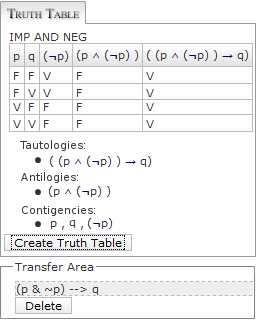
\includegraphics[width=0.34\textwidth]{f-4-truthTable}}
\\
\subfigure[\e{WFF Generator}]{\label{fig:generator} 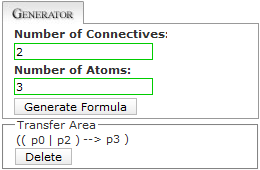
\includegraphics[width=0.34\textwidth]{f-2-generator}}
\qquad
\subfigure[\e{Tree Interaction}]{\label{fig:tree} 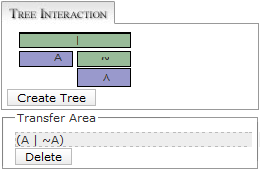
\includegraphics[width=0.34\textwidth]{f-5-treeInteraction}}
\caption{Some Learning Objects prototypes of \t{Logicamente}}
\label{prototipos-1}
\end{figure}


\noi $\bullet$  \e{Tree Interaction}: the formulas are data structures that corresponds to trees. This module makes these trees viewable, and allows the user to interact in various ways with theirs nodes and leaves of such trees. Many other uses are given in this module interact, view and interact with tableaux, resolution method and natural deduction. In the Figure \ref{fig:tree}, the module shows a generated tree representing the formula $(A \vee \neg A)$.


\noi $\bullet$  \e{Substitution Master}: implements a function that takes a formula in first order, a variable to be replaced and a term, and first of all, by checking if the term is free for the variable in the formula received
\footnote{A term  $t$  is \e{free for} a variable $x$ in a wff $\alpha$, if there is no ocurrences of $x$ in $\alpha$  in an scope of quantification, of $\forall y$ or $\exists y$, such that $y$ is a variable in $t$.}. If so, the replacement is made. Otherwise, the user is consulted if he desire to properly rename the bound variables of the formula to allow the replacement is performed. In the Figure \ref{fig:substitution}, we display the replacing of the variable $x$ by the term $f(a)$  in the formula $\forall y R(x,y)$, resulting in  $\forall y R(f(a),y)$.

\noi $\bullet$ \e{WFF Converter}: this module performs some conversions of formula necessary for the method of resolution in first order logic, through the manipulation of quantifiers and connectives in the appropriate reductions. The module accompanies, step by step, the conversion of a formula for the Conjunctive Normal Form (CNF)\footnote{ A formula is in Conjunctive Normal Form, if is a conjunction of subformulas such that each of the subformulas is a disjunction of literals and each literal is an atomic proposition, or the negation of an atomic proposition, i.e. has the form $p$ or $\neg p$.} and interactively transforms formulas for Prenex Normal Form (PNF)
\footnote{A formula is in prenex normal form, if has the following form: $Q_1 x_1...Q_n x_n \alpha$ such that $\alpha$ is a formula free quantified, $x_1,...,x_n$ are different variables and each $1\leq i \leq n$, $Q_i$ is $\forall$ or $\exists$.}. The module also receives first order formulas in PNF and enables application of the method of Skolemization\footnote{The name of the method is in honor of the mathematician and philosopher Thoralf Skolem (1887-1963). Skolemization means the elimination of existential quantifiers in closed formulas in PNF, where the variables are replaced by functions of choice and new symbols are introduced constants and functions.}.


\noi $\bullet$ \e{Resolution Game}:  implements the basic resolution method, assisting the student in eliminating complementary literals\footnote{ The resolution method is used to decide whether a sentence has a formula in CNF that is a theorem. If $\alpha$ and $\beta$ are basic clauses, with $p_k$ $\in$ $\alpha$ and $\neg p_k$ $\in \beta$, then the result of the rule Complementary literal elimination of $\alpha$ and $\beta$ -- concerning to $p_k$ and $\neg p_k$ --  is ($\alpha - \{ p_k\}) \cup (\beta - \{ \neg p_k\})$, such that $\gamma - \delta$  means the set of the diference between $\gamma$ and $\delta$, i.e. $\gamma - \delta \equiv \{ x | x \in \gamma$ e $x \notin \delta\}$.}.  The Figure \ref{fig:resolution} shows a instance of the resolution method for $\{ \alpha \vee \beta , \neg \alpha , \neg \beta \} \longmapsto \square $, concluding that  $\{\alpha \vee \beta , \neg \alpha , \neg \beta\}$ is a set of contradictory formulas.

\begin{figure}[ht]
\center
\subfigure[\e{Prenex Converter}] {\label{fig:prenex}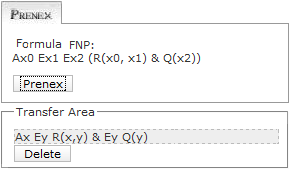
\includegraphics[width=0.34\textwidth]{f-6-prenexConverter}}
\qquad
\subfigure[\e{Skolemiser}]{\label{fig:skolemise} 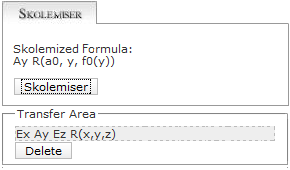
\includegraphics[width=0.34\textwidth]{f-7-skolemise}}
\\
\subfigure[\e{Substitution Master}]{\label{fig:substitution} 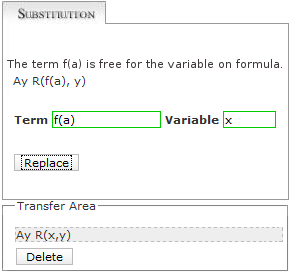
\includegraphics[width=0.34\textwidth]{f-8-substitutionMaster}}
\qquad 
\subfigure[\e{Resolution Game}]{\label{fig:resolution} 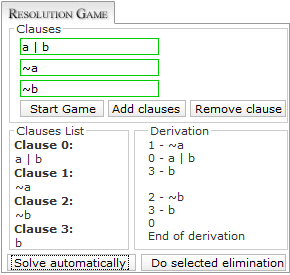
\includegraphics[width=0.34\textwidth]{f-9-resolutionGame}}
\caption{Others Learning Objects prototypes of \t{Logicamente}}
\label{prototipos-2}
\end{figure}


Our imediate goal is to add the following LOs, already implemented but not yet integrated to the \t{Logicamente}:

\noi $\bullet$ \emph{Small Counter-Model Builder}: implements a finite search engine of counter-models, i.e. a bounded model checker, receiving as input a number limited of objects, a collection of assumptions and a goal formula of conclusion.

\noi $\bullet$ \emph {WFF Diagnoser}: tests whether a expression is a well-formed formula and, in a negative case, it suggests some fixes. The module verifies if there is some redundant parentheses in the formula, besides it exposes various informations of well-formed formulas: its complexity, its set of basic atoms of subformulas among others properties.

\noi $\bullet$ \emph{WFF Translator}: the module create syntax for formulas and might to represent the connectives in different ratings symbols, images, HTML codes, codes in ASCII or \ LaTeX. Also with this module, its possible to translate formulas of different applications.

\noi $\bullet$ \emph{Tableaux Constructor}: implements the method of tableaux of first order logic, allowing the student to see the refutation tree and choose which rule to use.


\noi $\bullet$ \emph{Semantic Consequence Tester}: here the student can insert sets of propositional formulas and test step by step, the relation of semantic consequence involving the same. The module generates a counter-model whenever possible.


\noi $\bullet$  \emph{Theorem Proving Web System}: implements a demonstration assistant in Natural Deduction. We intend to develop this module integrating to our project the ProofWeb\footnote{ The \e{ProofWeb} is an opensource software for teaching Natural Deduction which provide a interaction between some demonstrators theorems (Coq, Isabelle, Lego) and an interface Web. It is available in \url{http://proofweb.cs.ru.nl/}.}.


%	\subsection{Organization and epistemic content of \t{Logicamente}}


	\subsection{Modeling presentation}



The \t{Logicamente} is implemented as a Web application in PHP language and AJAX technology, aiming that the system be available at anywhere and without require a previously installation. 
In Figure \ref{fig:formula}, we observe the model diagram currently implementated structures of propositional sentences, first-order propositions and their relationships between terms and functions.


All LOs presented above should cover both the classical first order logic as propositional logic. The set of LOs specified above must meet the following requirements:

\begin{itemize}
\item User Interface: For each LO, a user-friendly interface is implemented to provide easier and enjoyable to use. Besides that, the system has a tutor for the novice user can use the program and answer a few questions about the system.

\item Correction and optimization: we carefully analyse the implementation of all Learning Objects to maintain the correction of the implemented algorithms.
\end{itemize}


In the Figure \ref{fig:acti}, is shown the activity diagram of loading process of the Moodle, until the VLE is ready to be used. The activities take place in an order that begins with the connection to the database. The second step is to load the classes, note that the \t{Logicamente} is a module of Moodle and can be added to any course. In this point we assume that we have already loaded a course and registred his activities. After the Moodle and \t{Logicamente} are loaded, we can access the course in accordance with the kind permission of the user account. See Figure  the activity diagram.


The diagram of Figure \ref{fig:comp} presents the component view with the integration of Moodle and \t{Logicamente}. On the basis of Moodle we have the system with data access components, libraries, configurations and component view that calls the VLE. In the system we have an important component that is the setting that is requisite for this to work. Once set up the \t{Logicamente}, we will have access to all modules that access to the their libraries.


\begin{figure}[ht]
\center
\subfigure[\e{Component Diagram}] {\label{fig:comp}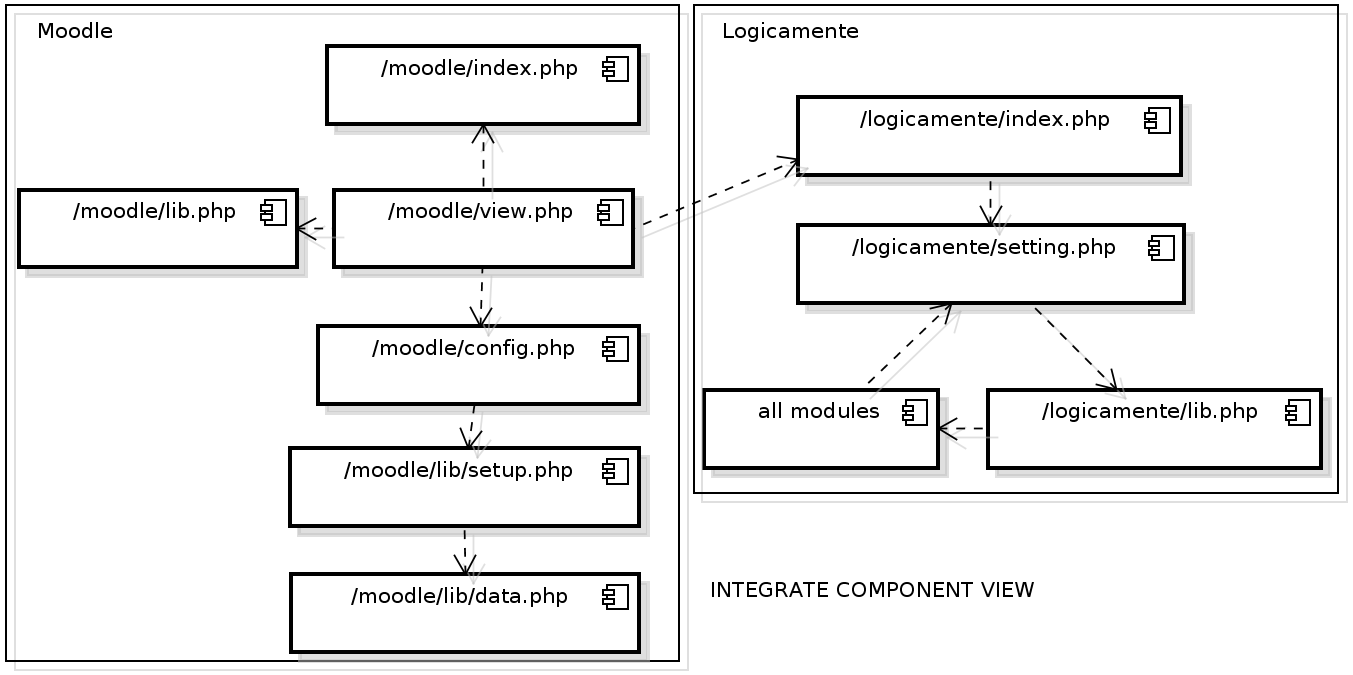
\includegraphics[width=0.65\textwidth]{f-component}}
\\
\subfigure[\e{Activity Diagram}]{\label{fig:acti} 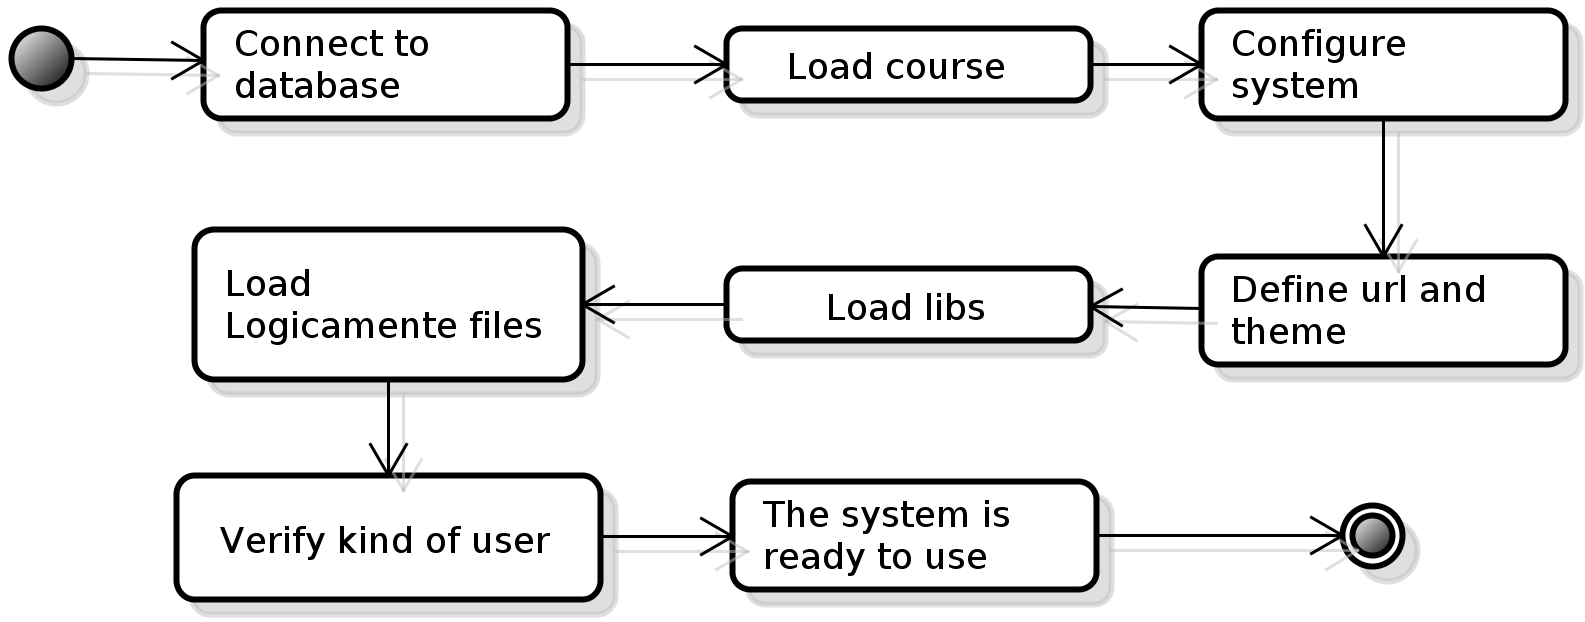
\includegraphics[width=0.48\textwidth]{f-activity}}
\quad
\subfigure[\e{Model Diagram implementing formulas}]{\label{fig:formula} 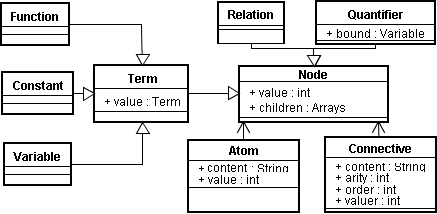
\includegraphics[width=0.45\textwidth]{f-diagrama-formula}}
\caption{Architecture Overview of \t{Logicamente}}
\label{prototipos-2}
\end{figure}





	













\section{Methodological Aspects: evaluation and monitoring of learning Logic}

\begin{flushright}
\scriptsize  

\e{It is by logic that we prove,\\
but by intuition that we discover.} \\
\t{--- Jules Henri Poincar�} \\
\e{In Science and Method (1908) translated by Francis Maitland (1914, 2007), 129.}
\end{flushright}

\noi Following the line argued by Antonia Huertas \cite{Huertas2007} to the teaching and learning logic -- identifing two paradigms of education, face-to-face and e-learning --, we agree that should be adopted teaching techniques for the course that use elements of both. For example, it is still difficult to have an evaluation method based only on the e-learning paradigm, then we must do activities in e-learning modality  and any test in the old model with paper and pen. 

However, the success of a model based on e-learning depends not only on techniques applied in most VLEs, after the adoption of this model is a constant need to improve the motivations to the student and the uses of process. The mains methodologies identified by \cite{Huertas2007} are: Instrumental, Interdisciplinary, Constructivism, Conceptual modeling, Personalization of the learning process, Workload adjustment and Continuous evaluation process. Our aim is to further examine these features applied into the project \t{Logicamente}.


In the \t{Logicamente}, the teacher have the control of students, classes, lessons and exercises. Besides, even the teacher have access to activity reports of students performance, also there is an agent for monitoring the learning modules and students activities of interactions with the OAS. In turn, the student is assessed by his performing with assigned lessons and have exercises related to LOs.

The LOs developed and presented aim to clarify the relationships between different approaches of logic, such as the semantic theory, the proof theory and others approaches of Logic applied. These different approaches will have their content associated with activities and challenges offered in Moodle, aiming a constructive process of teaching and learning Logic. The \t{Logicamente}, seeks to explore the potential offered by Web methodological, and also enable the implementation of different teaching styles of logic, without being restricted to particular styles of learning.


\section{Future Works and Final Remarks}


\begin{flushright}
\scriptsize
\e{``Contrariwise,'' \e{continued Tweedledee}, ``if it was so, it might be; \\
and if it were so, it would be; but as it isn't, it ain't. That's logic.''} \\
\t{--- Lewis Carroll} \\
\e{Through the Looking-Glass (1871).}
\end{flushright}

\noi Aiming to facilitate the reuse of LOs, the \t{Logicamente} use the standard IMS Learning Design (IMS-LD) to have their specified content and to ensure the sustainability of its resources \cite{IMS2003}. IMS LD is compatible with Moodle and is a framework used for the planning of new courses, support activities, organization of learning environments \cite{Souza2006}. On Figure \ref{fig:high-level} we present an overview of our system through the tool of editing and reuse of LOs, the ReCourse\footnote{Avaliable from \url{http://www.tencompetence.org/ldauthor/}.}.



\begin{figure}[htbp]
\centering
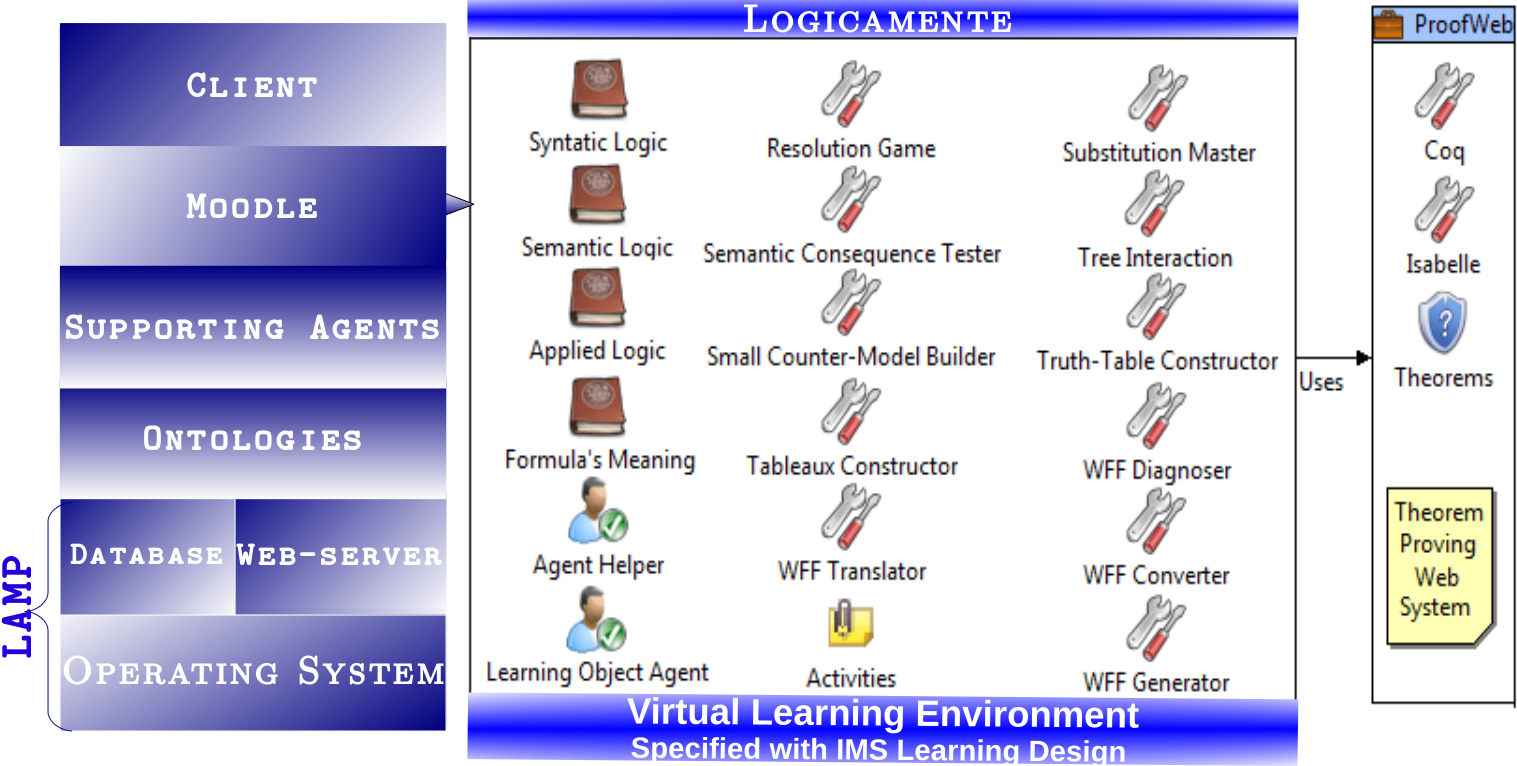
\includegraphics[width=13cm]{f-high-level}
\caption{High level presentation of \t{Logicamente}}
\label{fig:high-level}
\end{figure}

\noi A second point identified in \cite{Bittencourt2008} was that the teaching supported by computer can enjoy the benefits of semantic web. In this sense the \t{Logicamente} need to use Semantic Web techniques, to effectively manage organize and manage e-learning resources available according to peculiar necessities of both teachers and students, has been advocated by many authors. He presents the components of the Semantic Web-based Educational Systems (SWBES) as described in \cite{Bittencourt2008} are related to the roles mainly of users (teachers, learners, authors, groups, developers) to the educational resources, to the environment, to its to interface and the functionalities it does offer. The SWBES should include: ontologies, tutoring/pedagogical agents, semantically Described tools and services (better if they are web 2.0 based). Accordingly identified as a future goal to create ontologies for intelligent agents that can organize and manage learning resources in accordance with the special needs of each user.


Currently, the area of teaching Logic has a lack for a computational tool to explore other styles of learning and teaching. Although there are available tools for teaching logic, these applications do not represent virtual learning environments and really integrated interactively. In order to fill this need, we present the project \t{Logicamente}. In the present work, we have explained how the project was initially conceived from the work collaborative and learning based on implementation problems, finally it was presented  its learning objects implemented currently.



\bibliographystyle{sbc}
\bibliography{ref}

\end{document}


\begin{figure}[ht]
\centering
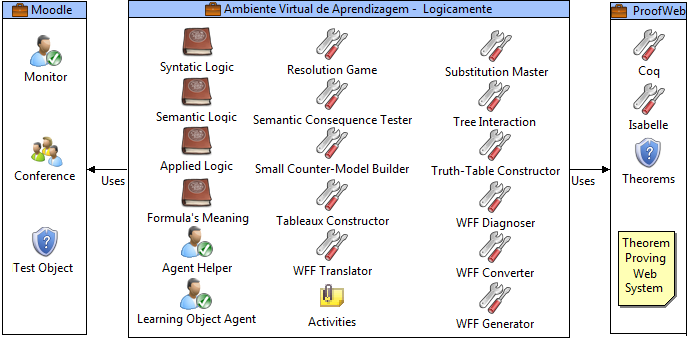
\includegraphics[width=13cm]{f-diagrama-ava}
\caption{Overview Diagram of VLE \t{Logicamente}}
\label{fig:ava}
\end{figure}






